\documentclass[12pt]{article}
\usepackage{graphicx}
\usepackage[hidelinks]{hyperref}

\graphicspath{ {./images/} }

\begin{document}

\title{Formulario Segnali}
\author{Giuliano Vallone}
\date{}
\maketitle

\tableofcontents
\newpage

\section{Software requirement Specifications}
\subsection{Introduction}
\subsubsection{Aim of the document}
\subsubsection{Overview of the defined system}
\subsubsection{Hardware and Software requirements}
\subsubsection{Related Systems, Pros and Cons}
\subsection{User Stories}
\begin{itemize}
\item As a player, I want to read the description of a challenge, so i can search for external material to study on for solve the challenge
\item As a player, I want to see a global scoreboard, so i can measure myself with other players on the platform
\item As an admin, I want to be able to change the flag of a challenge
\end{itemize}
\subsection{Function Requirements}
\begin{itemize}
\item The system shall provide a scoreboard accessible by all players
\item The system shall provide a login for non registered players
\item The system shall provide a description and a link for every attachment of the challenge when a player selects it
\end{itemize}
\subsection{Use Cases}
\subsubsection{Overview Diagram}
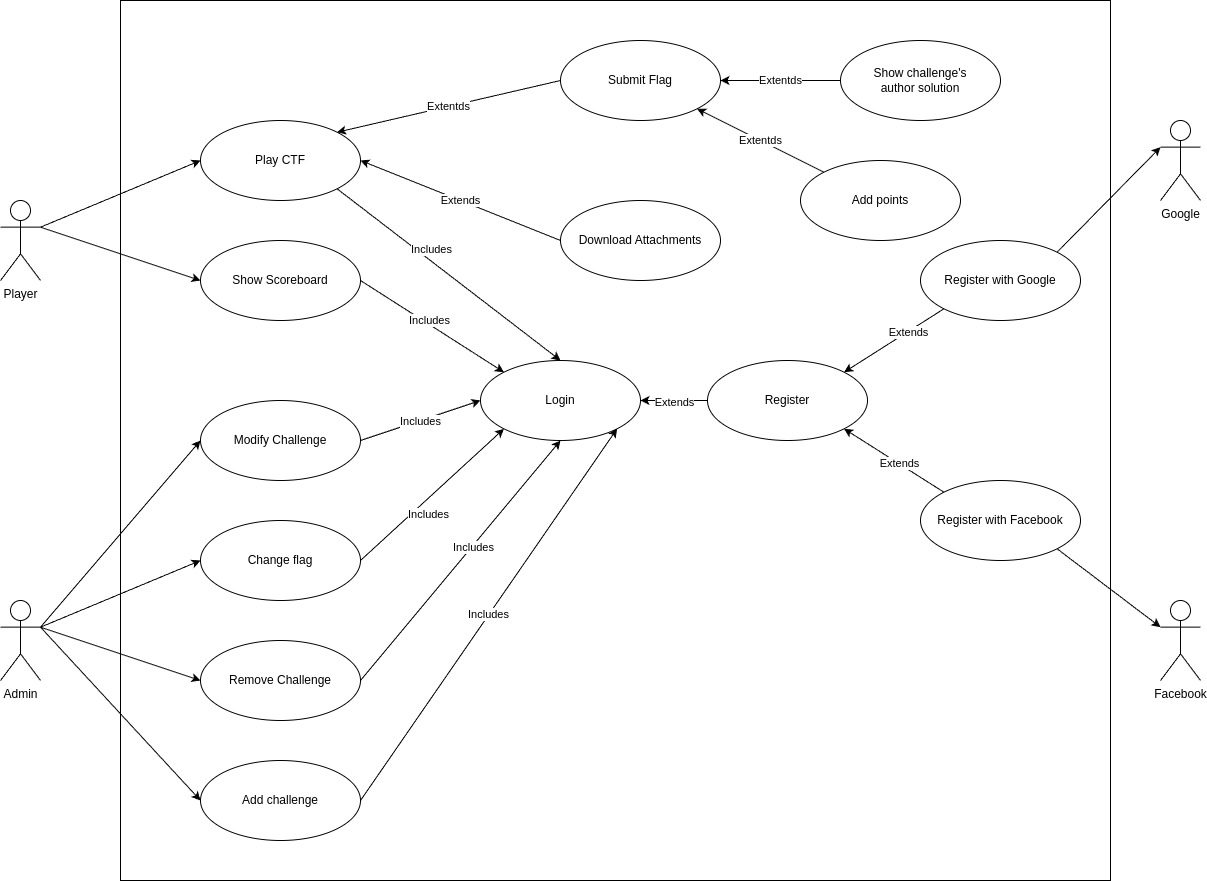
\includegraphics[scale=0.4]{Use Case Diagram.jpg}
\subsubsection{Internal Steps}
\section{Storyboards}
\section{Design}
\subsection{Class Diagram}
\subsubsection{VOPC}
\subsubsection{Design-Level Diagram}
\subsection{Design Patterns}
\subsection{Activity Diagram}
\subsection{Sequence Diagram}
\subsection{State Diagram}
\section{Testing}
\section{Exceptions}
\section{Persistance}
\section{Sonar Cloud}
\end{document}